\chapter{Background}
\label{chapter:background} 

This chapter will describe the main motivation and theoretical background behind our research. In a systematic stepwise approach we shall list and describe the main topics. We shall start with the motivation, inspiration and the partners of this thesis and then we shall try to explain the theoretical concepts with the reference to previous work done on the respective topics. For each topic we shall also describe how it has contributed for our research. 

\section{Smart grids }

Energy industry across the globe is facing numerous challenges. There is a huge pressure from regulatory authorities and environmental organizations to reduce carbon foot print, expand their renewable energy portfolios, and take energy conservation measures. The demand response (DR)\footnote{Demand Response(DR); Changes in electric usage by end-use customers from their normal consumption patterns in response to changes in the price of electricity over time, or to incentive payments designed to induce lower electricity use at times of high wholesale market prices or when system reliability is jeopardized.} and its impacts on consumer behaviour requires rapid adaptations in energy service providers business models. According to United States Federal Energy Regulatory Commission (FERC) , ``Demand response can provide competitive pressure to reduce wholesale power prices; increases awareness of energy usage; provides for more efficient operation of markets; mitigates market power; enhances reliability; and in combination with certain new technologies, can support the use of renewable energy resources, distributed generation, and advanced metering. Thus, enabling demand-side resources, as well as supply-side resources, improves the economic operation of electric power markets by aligning prices more closely with the value customers place on electric power''\cite{federal2008assessment}.  
Traditionally, power system participants have been strictly producers or consumers of electricity. The demand response and reliability issue with conventional electric power distribution models on consumer side are causing a major trend in motivating consumers to produce electricity at domestic level mostly using the renewable energy production methods.  `` Prosumer'' is an emerging term used for an economically motivated entity that: \cite{grijalva2011prosumer}
\begin{itemize}
\item Consumes, produces, and stores power,
\item Operates or owns a power grid small or large, and hence transports electricity, and
\item Optimizes the economic decisions regarding its
\end{itemize}

The current energy grids support unidirectional distribution models and are centralized in nature.  They are very limited to handle the prosumer needs. Line loses and hierarchical topology makes them less reliable. They usually become bottle neck when rapid adaptations are required for demand response. Farhangi, 2010 define smarts grids as ``The next-generation electricity grid, expected to address the major shortcomings of the existing grid. In essence, the smart grid needs to provide the utility companies with full visibility and pervasive control over their assets and services. The smart grid is required to be self-healing and resilient to system anomalies. And last but not least, the smart grid needs to empower its stakeholders to define and realize new ways of engaging with each other and performing energy transactions across the system'' \cite{farhangi2010path}.

In our research, we used data collected from smart metering devices as part of a pilot smart grid project. The data was used to generate analysis that recommends improvement for both demand and supply side to achieve energy efficiency as well as provide understanding to enable correct decision to adapt for demand response.


\section{CIVIS project}

CIVIS is the abbreviated name for ``Cities as drivers of social change'' project under European Union 7th framework. It is a part of the programme for optimising energy systems in smart cities. CIVIS project is a collaborative effort of 10 European universities) \footnote{1. Associazione Trento RISE, Italy 2. Aalto university, Finland 3. Imperial College London, UK 4. ENEL Foundation, Italy 5. Instituto Superior Técnico, Portugal 6.Karlsruhe Institute of Technology, Germany 7.Kungliga Tekniska Hogskolan, Sweden 8.SANTER REPLY SpA Italy 9.Nederlandse Organisatie voor toegepast Natuurwetenschappelijkonderzoek, Netherlands 10. Delft University of Technology,Netherlands  }. It aims to embed the social aspect into the advancements of energy technology. To unleash the full potential of this vision, smart grids need to be coupled with broader social and cultural considerations and understood as complex socio-techno-economic systems with multiple decision making layers that are in effect at the physical, cyber, social, and policy \cite{civisproposal}.

ICT acts as one of the main enabler of smart grids,  distributed  and bidirectional information flow models. On the other hand ICT also provides a lot of new mediums for social aggregation e.g. internet based social media. CIVIS projects tends to connect these two different dimensions with innovative ICT solutions. An integrated approach to energy efficiency is the basic manifesto of CIVIS project. \cite{civisproposal}

Understanding energy usage patterns and benchmarking energy efficiency performance of small units within cities are some preliminary items in list of CIVIS objectives. Within scope of our research we analyse energy data to understand the consumption patterns and try to evaluate various factors that can effect directly or indirectly on the usage patterns. We also try to classify the building on basis of energy efficiency and try to test the sensitivity of energy efficiency with respect to factors that can cause shift in usage patterns. For the CIVIS project aim of social aspect integration, we also present an ICT application framework that can be used to collect and analyse social media data. However the analysis of that data is not within the scope of this research. 


\section{Green campus initiative}

Green campus initiative is a project by VTT  ``Technical Research Centre of Finland'' . It is part of EcoCampus 2030 program. EcoCampus is an attempt to increase energy efficiency in districts and buildings by innovative management and control systems capable to optimize the local consumption without compromising the indoor environment, occupant comfort and building performance, and by introducing new ICT enabled business models \cite{ greencampus}. The vision of the program is to realize a net zero energy model for a world class research, development and educational facility. Program focuses on co-designing this model with user by educating them and then collecting feedbacks for improvement. The main aim is to gain energy efficiency by building infrastructure in the building units that can make them self sustain for future requirements. The aim is build to build a performance based ecosystem that can help both consumers and producers to adapt with demand response.

Green campus initiative is a pilot project for EcoCampus program  in which VTT has installed smart devices inside Aalto University, Finland campus building in cities of Espoo and Helsinki. These specialized devices contained smart metering for energy consumption and indoor environment monitoring sensors.  The data used for analysis in our research was collected from a subset of buildings as test sites of this project. The data includes hourly consumption of electricity and electricity used for heating. For one of the test sites VTT provided us the data with device level energy consumption details i.e. electricity used by different home appliances. This was achieved using smart NIALM \footnote{ NIALM stands for non-intrusive appliance load monitoring,  is a process for analysing changes in the voltage and current going into a house and deducing what appliances are used in the house as well as their individual energy consumption }\cite{ hart1992nonintrusive} meters that can distinguish between different electric devices used on basis of their signal thumb print.

Apart from providing the data, VTT green campus researchers have also helped us in formulating the use cases for this thesis research.


\section{Big data analytics}

Big data analytics is the application of advance data analytics techniques on large volumes of data. Advance analytics is a generalized term used for data analysis techniques like statistical analysis, data mining, machine learning, natural language processing, text mining and data visualization etc \cite{russom2011big}. Although volume of the data is a widely used factor for qualification of a data set as big data but when it comes to big data analytics there few other important attributes i.e. variety, velocity, valuation and veracity. The concept of 3Vs (volume, variety and velocity) of data was first given by an analyst, Doug Laney from Gartner  in a 2001 MetaGroup research publication, ``3D data management: Controlling data volume, variety and velocity''\cite{laney20013d}.  Gartner used this concept to formulate a data magnitude index that can support decision making for selection of the solutions for tackling big data challenges. This concept is shown in figure~\ref{fig:3Vs} below

\begin{figure}[ht]
  \begin{center}
    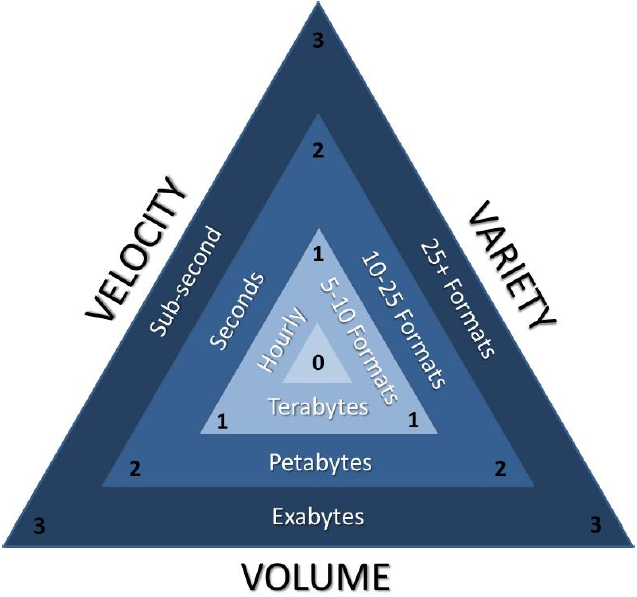
\includegraphics[width=0.7\textwidth]{images/3Vs.png}
    \caption{Gartner 3Vs of data and data magnitude index \cite{laney20013d}.}
    \label{fig:3Vs}
  \end{center}
\end{figure}

Number 0 to 3 represents the scale of data that you perceive on each dimension. Adding them together for a big data case can provide the data magnitude index. This method provides some basis for quantifying the data as big data, However it is not providing a definitive model as it allows presumptions to scale the data. Valuation and veracity are two other factors that are being used widely along with Gartner's 3V. Valuation supports the decision making by considering the value of outcomes against the efforts required to collect, manage, process and analyse huge amounts of data.  While veracity refers to ambiguity in the data that can cause complexity. There is no standard definition of big data but most of the attempts to define big data can be associated with these five factors that we have discussed.

As a matter of fact, we are not attempting to provide a definition of big data as part of this thesis or stating any criteria for qualification of a data set as big data. Instead we shall be proposing an advance analytics model that should be capable enough to handle big data as well other smaller data sets on need basis. The modular architecture of the model platform can be tweaked to handle volume, variety, velocity, and veracity on need basis while trying to maximize the valuation for the use case. In following subsections we shall discuss some of the relevant technological advancements that enables to handle the mentioned challenges of big data analytics. These concepts, tools and techniques are also used in developing the data analytics platform and performing the analysis for our thesis research.

\subsection{Parallel batch processing with MapReduce and Hadoop} \label{mapr} 
It is hard to predict the size of data and computing power required to pocess it when dealing with big data. Scaling up \footnote{When the need for computing power increases, a single powerful computer is added with more CPU cores, more memory, and more hard disks and used in parallel.}is an option that is always bounded by some maximum capacity limits. Also specialized hardware to scale up for higher capacity usually gets very expensive. So the viable option is to scale out \footnote{When the need for computing power increases, the tasks are divided between a large number of less powerful machines with (relatively) slow CPUs, moderate memory amounts, moderate hard disk counts.} using required number of smaller machines with relatively low computing resources in parallel. We need a system that can handle large scale parallelization. From programming point of view managing parallel running processes on different machines while ensuring low failure rate is a tough job. So the desired system should provide programmers an abstraction from lower level system details to enable rapid and fault tolerant development for big data processing.  MapReduce is a parallel batch processing framework developed at Google for the purpose of web indexing. The concept of MapReduce was published by Jeffrey Dean and Sanjay Ghemawat in 2008 within their research paper ``MapReduce: simplified data processing on large clusters''  \cite{dean2008mapreduce}. This paper describes MapReduce as ``programming model provides a map function that processes a key/value pair to generate a set of intermediate key/value pairs, and a reduce function that merges all intermediate values associated with the same intermediate key. Programs written in this functional style are automatically parallelized and executed on a large cluster of commodity machines. The run-time system takes care of the details of partitioning the input data, scheduling the program's execution across a set of machines, handling machine failures, and managing the required inter-machine communication''.

Hadoop is the open source implementation of MapReduce developed by Doug Cutting and Mike Cafarella. It was initially created in 2005 to support an open source search engine but then adapted to the published MapReduced framework \cite{dean2008mapreduce}. It was released by Apache foundation. Apache foundation has also built many supporting tool around Hadoop framework to support end to end big data analytics ecosystem e.g. Apache flume for data collection, Hadoop File system (HDFS) for storing, Apache Pig and Hive for processing, Apache Mahout for machine learning etc. We have used some of these tools within scope of our research. 

MapReduce and Hadoop are batch processing frameworks that empower processing of large volumes of data using commercial grade low cost computing infrastructure. So it supports volume and valuation directly. Variety can also be supported with support of all format files into associated files system e.g. HDFS.  Veracity is subjected to supported tools like data collection or data mining tools. Support for such tools is available in Apache hadoop e.g. Flume, Mahout etc. Velocity however is the only feature that a batch processing framework like MapReduce and Hadoop cannot handle. The next subsection answers the question of velocity.

\subsection{ Real time big data processing }
Real time data processing is generally associated with live streams of data. Real time data can be processed and analyzed on arrival or it can be buffered for small intervals to provide near to real time analysis. However in many modern data applications instantaneous data needs to be analysed in context to large volumes of historic data. To apply advance analytics models like machine learning active feedback loops are also necessary.  Even stored (non live data) big data, applications require data processing system to answer queries very fast. To fulfil these industry driven requirements technology is in rapid advance mode. In last twelve to eighteen months we have seen software like YARN (Hadoop 2.0), storm, spark, shark , cloudera impala etc with near to real time processing capabilities. On top of it tools like Mlbase and cloudera oryx have started to enable real time advance analytics. Most of these system, frameworks and tools are being developed as the evolution path for MapReduce and Hadoop. All of them have their own purpose, strengths , and limitations. They are mostly used in combinations based on use cases. We shall not be discussing or comparing these systems and tool. Instead, in this article we shall be briefly discussing the two prevailing architectural constructs that can enable real or near to real time big data processing.

\subsubsection{ Lambda architecture}
Lambda architecture presents a hybrid model by using fast stream processing together with relatively slow parallel batch processing.  It was developed by Nathan Marz on the basis of knowledge and experience he gained from his work with large data sets at Twitter Inc. His approach decomposes data processing system into three layers i.e. a batch layer, a serving layer and a speed layer. The stream of data is dispatched to both the batch and speed layers. Batch layer manages the historic data set and pre-compute the batch views. Serving layer indexes the batch views so the queries can be served with low latency as compared to traversing through complete data set. Speed layer deals with the recent data thus compensates for the change of data sets during updates of serving layer. An answer to the query is the merged view batch view and the real time view.\cite{marz2013big}\cite{lambdaarch} 

Figure~\ref{fig:lambda} below show the Lambda architecture. Lambad architecture can be implemented using combination of systems and tools e.g.Apache Hadoop along with Apache Storm.
\begin{figure}[ht]
  \begin{center}
    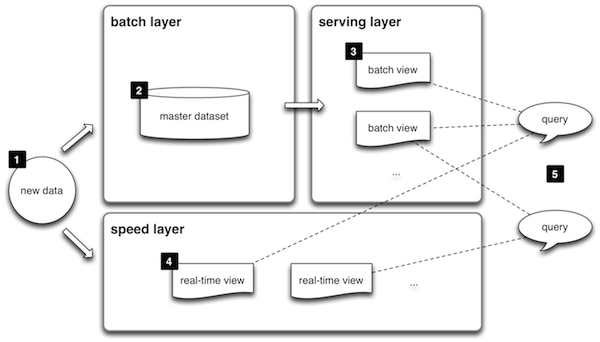
\includegraphics[width=\textwidth]{images/lambda.png}
    \caption{Lambda Architecture \cite{lambdaarch}.}
    \label{fig:lambda}
  \end{center}
\end{figure}

\subsubsection{Massively parallel processing - MPP databases and query engines}\label{mpp}
MPP based architectures use multiple independent computing resources like severs, processors and storages to execute processing jobs in parallel. Most of the MPP based database approaches implements shared nothing (SN) architecture i.e. a distributed computing architecture in which each node is independent and self sufficient and there is no point of contention across the system. The SN concept for databases was first presented by Michael Stonebraker at University of California Berkeley in 1986 \cite{stonebraker1986case}.. The SN databases have been very popular in commercial application primarily because of the high scalability offered by this architecture. Teradata warehousing solutions has been using SN database architectures extensively. Greenplum is an example for open source SN database.

Despite high scalability and other positive aspects, SN databases needs a lot of manual work in terms of partitioning the data, tuning the data and load balancing etc. So usually maintenance such database systems is expensive. MapReduce and Apache Hadoop ecosystem provides high level of automation along with scalability, flexibility and fault tolerance. However parallel batch processing is not as fast SN based MPP databases. Merging both the models solves can solve all these issues. Cloudera Imapala is one of the example of a MPP based on-line query engine that runs natively on top of Hadoop \cite{ clouderaimpala}. It can provide MPP like query response time performance with processing power and flexibility of Hadoop. For our research we have used Cloudera Impala for handling near to real time velocity for big data processing.

\section{Energy efficiency and eco-effeciency}
In previous sections of this chapter, we have highlighted the importance of energy conservation. We discussed the advancements in pervasive smart energy device and grids and their role in improving energy efficiency.  We have also discussed the need for collecting and processing large volumes of data from smart energy devices and the available solutions. In this section we shall explain the main motivation and the theoretical concept behind data analysis part of our research.  

Unprecedented challenges arising from increasing dependency on conventional energy are part of a global phenomenon. Improving energy efficiency is an important mean to tackle these challenges. Like other economies, European Union is also putting a lot of focus on energy efficiency to ensure energy supply security  by reducing primary energy consumption and decreasing energy imports. It helps to reduce greenhouse gas emissions in a cost- effective way and thereby to mitigate climate change \cite{eu2012ee}. Member states agreed to reduce 20\% of the EU's primary energy consumption by 2020 in European Union of council March, 2007.  EU's Energy Efficiency Directive 2012 \cite{eu2012ee} defines energy efficiency as the ratio of output of performance, service, goods or energy, to input of energy. This definition was first discussed in 2006 in European commission action plan for energy efficiency. This generic definition covers all major aspects of the energy efficiency i.e. production, distribution, consumption and the value created in comparison to the resources consumed during the whole process.  However, To develop a methodology for measuring energy efficiency and to evaluate the savings, project ``Measuring and potentials of energy efficiency (EPO)'' was started in 2008\cite{arundel2009measuring}. As part of this project VTT published a report ``Measuring energy efficiency Indicators and potentials in buildings, communities and energy systems''\cite{forsstrommeasuring}. This report presents the model for calculating energy efficiency and its correlation with environmental factors.  VTT's research presented in this report considers energy efficiency as a subset of larger eco-efficiency. The ecological factors that can affect energy efficiency are e.g.  Temperature, CO2, NOx,SO2 etc. The ecological efficiency itself is a way of measuring sustainable development. VTT summarizes the whole ecosystem in Figure~\ref{fig:eco-effeciency} below

\begin{figure}[ht]
  \begin{center}
    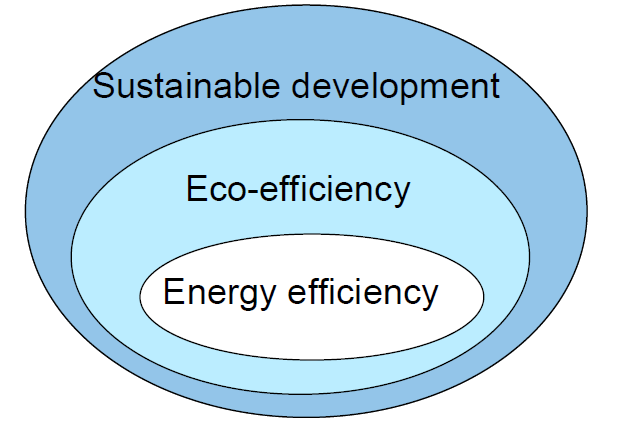
\includegraphics[width=0.8\textwidth]{images/eco-effeciency.png}
    \caption{ Energy efficiency, eco-efficiency and sustainability\cite{forsstrommeasuring}.}
    \label{fig:eco-effeciency}
  \end{center}
\end{figure}

The concept of eco-efficiency provides the basis for data analysis in our research. We have applied basic and advanced analytics techniques on data sets collected from building units that are part of VTT's green campus initiative pilot project with consideration of eco-efficiency model presented in VTT's report. We calculated energy efficiency of  the buildings on basis of formula deduced in Chapter 5 (equation 5.1 and 5.2) of the VTT's  report \cite{forsstrommeasuring}.
\begin{equation}
Energy\;efficiency\;of\;a\;building  =  \frac{Energy\;consumed}{Built\;area}
\end{equation}  

In case of a specific energy consumption (SEC) \cite{forsstrommeasuring} equation 2.1 can be written as 
\begin{equation}
SEC  = \frac{Q}{A}
\end{equation} 
Where Q denotes the consumption for a single energy type for example electricity and A is the built area in meter square. In subsequent sections we shall be  referring to these equations when we try to identify the usage patterns on building level, discuss the relevance of  energy efficiency with these patterns and then discuss a model for classifying buildings on energy efficiency .

\section{Daily consumption patterns, base load and user load}\label{daily}
Daily consumption pattern of a building unit corresponds to the respective usage of the building. Understanding daily usage patterns can help in identifying the optimization point for improving the energy efficiency of that building unit. Base load of a building is one important metric that can be detected through observing the daily consumption. Base load is the consumption that takes place regardless of the actual use of the building and of the user's energy consumption\cite{forsstrommeasuring}. It is the permanent minimum load that a power supply system is required to deliver. The base load is usually caused by the continuous consumption for building maintenance like air conditioning, ventilation, or night time lighting. Sometimes base load also include some energy consumption by functional components inside building like computer servers, lab equipments, and refrigerators etc. However VTT differentiate this load from user energy load that is characterized by the direct involvement of the users of a building. For example an office building that has peak load during day time because user  are using various additional appliances like personal computers, coffee makers, lights etc compared to base load that is generated during night time when office building is not in use. Figure  ~\ref{fig:baseload} illustrates the concept of base load and user load.
\begin{figure}[ht]
  \begin{center}
    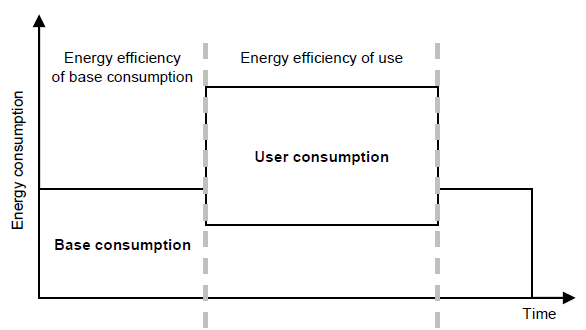
\includegraphics[width=0.8\textwidth]{images/baseload.png}
    \caption{ Base load , user load and energy efficiency \cite{forsstrommeasuring}.}
    \label{fig:baseload}
  \end{center}
\end{figure}

Energy efficiency of base consumption and energy efficiency of user load are shown in figure ~\ref{fig:baseload} can be calculated using equation 2.1 or 2.2. This provides a weighted metric that can be benchmarked and compared. It can help to narrow down scope of research by referring to problematic buildings and their issues.

\section{Energy consumption seasonal patterns}\label{seasonal}
Energy consumption has high dependency on seasonal factors like weather. The energy consumption trends vary with outside temperature. Among other things electricity or the other energy types required for the air conditioning in the buildings is major variable factor dictating the trends. Due to regional weather differences the seasonal energy consumption patterns are also different for different regions e.g. in cold regions of the world energy consumption surges in winters while in warmer regions energy consumption increase is expected in summers because of the air conditioning requirements. Energy service providers usually conduct demand planning with consideration of seasonal trends.Considering seasonal trends is also very important while optimising for gaining energy efficiency. 

In scope of our research we have also analysed the seasonal trends. It was not hard for us to perceive the trends while knowing the weather trend for localities of our test building. However, the interesting use case in our research was to check the sensitivity of other consumption patterns and analysis results against the seasonal trend. This will be more explained in the later part of document where we shall discuss the results of our analysis.

Previously, there have been many studies for both daily and seasonal trends in energy consumption. Due to regional differences in trends, many of these studies focused on consumption patterns within a country. Geoffrey K.F. Tso et. all, 2003\cite{tso2003study} and Yigzaw G. Yohanis et. all 2007\cite{yohanis2008real} study the energy consumption pattern in Hong Kong and United Kingdom respectively. Buildings units e.g. residential houses apartments and commercial offices etc were considered as basic unit of analysis. Yigzaw G. Yohanis et. all methodology resembles most to our approach as they considered ecological factor along with energy efficiency calculated in similar way as equation 2.1 and 2.2. As discussed before, the main purpose of VTT's green campus initiative under EcoCampus 2030 plan is to develop a highly efficient model ecosystem for energy production, distribution and consumption that can be expanded further to any scale. Alligned to this goal, we have attempted to provide a data analysis model that is not specific to certain geographic locations. However detailed study is required for adapting such generic models to region specific requirements. In our research we have also attempted to classify the buildings on basis energy efficiency that is explained in next section.

\section{Classification of buildings based on energy efficiency}\label{classify}

Earlier we mentioned that quantifiable energy efficiency through equation 2.1 and 2.2 can be used as a metric for benchmarking and comparison. For energy service providers, governmental energy regulatory agencies or research institute like VTT, it is very important to identify the problematic consumption units in larger number of highly optimized or average performing consumption units.Classification of these units into similarly performing groups can help them to narrow down the focus on problematic units. Sometimes it can also help in understanding the good practices applied by certain consumptions unit that has improved their energy efficiency performance.
  
Classification for fault detection analysis of a building energy consumption has been used previously as well. Xiaoli Li et. all, 2010 used classification along with outlier detection mechnism to identify the energy inefficient building \cite{li2010classification}.They provide a step wise approach to extract the features (types of energy, trends etc) from the data collected as a time series. Then detect identify the daily usage patterns using auto regression technique and pass the results to benchmark against any outlying data point that can refer to faulty behaviour. Imran Khan et all. 2013, proposes different clustering techniques to group building with similar level of energy efficiency together\cite{khan2013fault}. In our research we used a hybrid method using feature extraction and trend detection techniques like Xiaoli Li et. all\cite{li2010classification} and then applied a clustering technique proposed by Imran khan et. all \cite{khan2013fault}. The clustering technique that we used is called K-means clustering. It is explained in the next subsection of this article. 

\subsection{K-means clustering}
K-means is an algorithm for cluster analysis. In context to machine learning cluster analysis or clustering is an unsupervised task of grouping a set of objects in a way that objects in same group are similar to each other more than the objects in other group. K-means algorithm clusters the set of objects i.e. energy efficiency values in our case into predefined number of classes. We shall term these values as data points. K represents the number  of cluster and groups that we can set in start of the process. K-means means algorithm was first proposed by Stuart Llyod in 1957\cite{lloyd1982least} but the k-means term was first used by James Mcqueen in 1967\cite{macqueen1967some}. There have been many  adaptations and optimizations in Lloyd's basic algorithm. K-means algorithm today has many variants like Fuzzy C-means clustering, k-medoids and spherical means etc. Even for original Lloyd's algorithm there has been some modification in methodology. Two very commonly used methods are Forgy method \cite{forgy1965cluster} and Hartigan-Wong method\cite{hartigan1979algorithm}. In our approach we are using Hartigon-Wong method. We shall also use some references from Forgy method when explaining the K-means algorithm. 

K-means groups the data points in cluster with a logical centre point. The aim of the K-means algorithm is to divide data points in certain dimensions into K clusters so that the within-cluster sum of squares is minimized \cite{hartigan1979algorithm}. Lets assume if we want have K cluster for data points  D = \(\{x_1,x_2,\dotsc,x_n\}\) in d dimensions then
\begin{align*}
x_{i}& \in R ^{d}
\end{align*}
 
K-means algorithm uses following steps to cluster data into groups\cite{ng2000cs229}.
\begin{enumerate}
  \item Initialize the centroids randomly for each K i.e. for each group. 
  \item Data points are assigned to closest centroid.
  \item Move the centroids to the mean of the data points assigned to that cetroid in step 2.
  \item Repeat 2 and 3 till convergence Convergence means that values stop changing in further iterations.
\end{enumerate} 

Mathematically randomly initialized centroid are  
$${\mu_1,\mu_2,\dotsc,\mu_k}  \in R^{n}$$


If \(c^{i}\) is the distance of centroid to assigned data point then Step 2 and 3 with recursive distance minimization and mean adjustment can be explained as 

For every i, set 
\begin{equation}
c^{i} := \arg\min_j || x^{i} - \mu_j||^2
\end{equation} 
The equation above used Euclidean distance formula for calculating distance between centroid and data point. 

For every j, set
\begin{equation}
\mu_{j} := \frac{\sum\limits_{i=1}^n 1\{c^{i} =j\}x^{i}}{\sum\limits_{i=1}^n 1\{c^{i}=j\}}
\end{equation}

The input to k-means is a set of feature vectors along with the number of clusters required. In our case we shall be have two feature hence two dimensional matrix of energy efficiency values for electricity and electricity used for heating. Before inserting data to k-means it is required to set the similar scale for features as well set the standard variance to avoid errors in the results. We required to classify pilot site buildings into four groups with High efficiency, moderate efficiency, low efficiency and poor efficiency classes. So we have set K value as 4.

\section{Forecasting the energy consumption}\label{predict}
Estimating equipment specific energy consumption has been a key focus area for energy service providers. It can help in demand planning, load forecasting, and understanding end user behaviour.  Energy service providers can design better service offerings for their consumers. Unit energy consumption (UEC) is a term generally used for estimating equipment specific energy consumption. It is the average annual amount of energy consumed by a user device. Conditional demand analysis (CDA) model has been one the most commonly used method for UEC estimations. K. H. Tiedemann, 2007 explain CDA as a multivariate regression technique which combines utility billing data with weather information and customer survey data to produce robust end-use energy consumption estimates\cite{tiedemann2007using}. As part of the green campus project VTT has installed used state of the art nonintrusive load monitoring (NIALM)\cite{hart1992nonintrusive} devices that can distinguish between the usage of different electric devices on basis of changes in voltage and electricity. 

We are using the data collected by a NIALM device installed in one of a residential apartment included in VTT's pilot test sites. In our analysis of this data we are not using CDA. However we shall be using auto regression along with concept of moving averages in form of a model known as ARIMA model to estimate the future consumption of a device depending on the previous usage. This is an example of quantitative forecasting. Before we go to discuss about ARIMA models it is important that we briefly discuss the basic conditions for quantitative forecasting and the time series analysis as foundation for prediction model based on ARIMA.
\subsection{Main conditions and Steps for Quantitative Forecasting}\label{conditions}
Rob Hyndman et all, 2014 discuss two main conditions for application of quantitative forecasting\cite{hyndman2014forecasting} in their book ``Forecasting: Principles and Practice''.
\begin{enumerate}
\item numerical information about the past is available.
\item it is reasonable to assume that some aspects of the past patterns will continue into the future.
\end{enumerate}
In case the conditions can't be met then qualitative forecasting is the only option. However, the qualitative forecasting is not in scope of our research for this thesis. In the same book authors mention following five step approach for solving forecasting problems.
\begin{enumerate}
\item Problem definition
\item Information gathering that includes statistical data collection.
\item Exploratory analysis of the data to evaluate the structure of the data and observing relationship between different variables.
\item Choosing and fitting the forecasting model. The model depends upon the relationships between variables. Every model has its own construct. So data needs to be fitted to that construct before applying that model. We shall discuss it more in data analysis part of tis document.
\item Using and evaluating forecasting model. It generally includes comparison of results after applying different models.  
\end{enumerate}    

\subsection{Time Series Analysis}
Time series is the sequence of a random variable collected over time. Among other examples of time series data, energy consumption data from metering devices can also be collected periodically hence constituting a time series. Comparison of a single time series at different point in times is termed as time series analysis \cite{box1976time}. A time series usually consists of a deterministic component and a random component\cite{mujumdarstochastic}. So if \(X_{t}\) is a time series data then we can have 

\begin{equation}
X_{t}= d_{t}\;+\;\epsilon_{t} 
\end{equation}  

where \(d_{t}\) is the deterministic component and \(\epsilon_{t}\) is the random component. The deterministic component itself can be in form of trends, periods, and jumps etc. Figure ~\ref{fig:time_series} illustrates the examples of different time series. In each illustration there is atleast one stochastic random component with and without deterministic components. 
\begin{figure}[ht]
  \begin{center}
    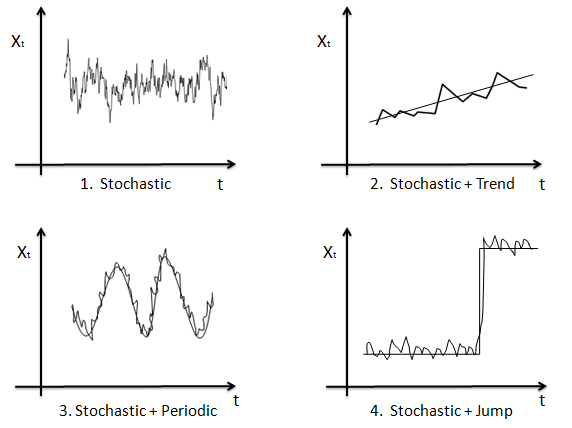
\includegraphics[width=0.8\textwidth]{images/time_series.png}
    \caption{ Time Series types\cite{mujumdarstochastic}.}
    \label{fig:time_series}
  \end{center}
\end{figure}  

In figure ~\ref{fig:time_series} illustrations 2,3 and 4 contain a deterministic component with a random component. In terms of prediction even the random component can be estimated using the deterministic component. However for stochastic random time series data without any deterministic component it is very hard to predict anything accurately. The time series with no predictable pattern is generally termed as stationary time series. We shall be discussing this in details during the  analysis part of this document.  

 
\subsection{Autoregression, Moving Averages and ARIMA Models} \label{ARIMA}    
 Rob Hyndman's book ``Forecasting: Principles and Practice''\cite{hyndman2014forecasting} is the main reference for this section. 
 \subsubsection{Regression}The concept behind basic regression techniques for forecasting is that we try to forecast a variable `y' on the basis of another variable `x'. For example a liner regression model forecast y assuming it has a linear relationship with  variable x e.g. as in equation below.
 $$ y = \beta_{0}\;+\;\beta_{1}x\;+\;\epsilon $$
 Parameter \(\beta_0\) and \(\beta_1\) represents the intercept and slope respectively for the line representing  the linear relationship.\(\beta_0\) represents the predicted value when x is 0. Linear regression for time series analysis can be written as 
 $$ Y_{t} = \beta_{0}\;+\;\beta_{1}x_{t-1}\;+\;\epsilon $$
 Here \(Y_{t}\) is the estimate with past value of \(x_{t}\) i.e. \(\{x_1,x_2,\dotsc, x_{t-1}\}\) . using differencing\footnote{The differences between consecutive observations} error \(e_{t}\) in estimation can be calculated as
 \begin{equation}
 e_{t}\;=\; X_{t}\; -\; Y_{t}\;=\; x_{t}\; -\;\beta_{0}\;-\;\beta_{1}x_{t-1}\;-\;\epsilon
 \end{equation}
 \subsubsection{Autoregression}  
 Autoregressive model is based on the concept of a variable regressing on itself. For autoregression we can drive equation as
  \begin{equation}
  x_{t}\; =\;\beta_{0}\;+\;\beta_{1}x_{t-1}\;+\;e_{t}\;+\;\epsilon
  \end{equation} 
  The aim for good estimation is to select value of \(\beta_0\) and \(\beta_1\) that can minimize the sum of square of errors. Above equation can be used to estimate the value based on first previous value. But in case we want to estimate based on multiple previous values e.g. `p' values then we can write it as 
 \begin{equation} \label{AR}
  x_{t}\; =\;c\;+\;\beta_{1}x_{t-1}\;+\;\beta_{2}x_{t-2}\;+\;\dotsc\;+\;\beta_{p}x_{t-p}\;+\;e_{t}\;+\;\epsilon
 \end{equation}
 
 We just replaced \(\beta_0\) with a constant c as it is a constant value. Adding the summation to the historic values we can write 
 
$$
x_{t}\; =\;c\;+\;e_{t}\;+\;\sum\limits_{i=1}^p\beta_{i}x_{t-i}
$$
we have also taken out the random component \(\epsilon\) that does  not meet the basic conditions for forecasting as described in subsection \ref{conditions}. The model presented  in equation \ref{AR} is referd to as AR\((p)\) model. 
\subsubsection{Moving Averages}
 Moving averages model use past forecast errors in regression like manner to forecast future time series values instead of using past time series values as in autoregression. Matehmatically model can be explained as
 \begin{equation}\label{MA}
 y_{t}\; =\;c\;+\;e_{t}\;+\;\theta_{1}e_{t-1}\;+\;\theta_{2}e_{t-2}\;+\;\dotsc\;+\;\theta_{q}e_{t-q}
\end{equation}
OR
$$
y_{t}\; =\;c\;+\;e_{t}\;+\;\sum\limits_{i=1}^q\theta_{i}e_{t-i}
$$
The model presented  in equation \ref{MA} is termed as MA\((q)\) model.In this model each value of \(y_t\) can be thought of as a weighted moving average of the past few forecast errors.
\subsubsection{ARIMA Model}
ARIMA stands for Auto-Regressive Integrated Moving Average. As the name suggests it is the combination of autorgresion and moving average models. ARIMA is one of the most commonly used forecasting technique. ARIMA model can handle time series data with and without seasonality. We shall be discussing non-seasonal ARIMA because of the nature of the data we shall be processing in our analysis. The nature of the data will be discussed in data analysis part of this document. So combining the autoregression and moving averages using equation \ref{AR} and \ref{MA} we can have 
\begin{equation}\label{ARIMA1}
 y^\prime_{t}\; =\;c\\;+\;e_{t}\;+\;\phi_{1}y^\prime_{t-1}\;+\;\dotsc\;+\;\phi_{p}y^\prime_{t-p}\;+\;\theta_{1}e_{t-1}\;+\;\dotsc\;+\;\theta_{q}e_{t-q}
\end{equation}
In this equation \(y^\prime_t\) is the difference series. This constitutes ARIMA\((p,d,q)\) model where
\begin{itemize}
\item p is the order of autoregression.
\item d is the number of non seasonal differences.
\item q is the order of moving averages.
\end{itemize}
Now to simplify the complex time series equation back shift notations are usually used e.g. \(y_t-1\) can be denoted by \(By_t\) i.e.
$$By_{t} = y_{t-1}$$
AND
$$B(By_{t}) = B^2y{t} = y_{t-2}  $$
AND 
$$ y_{t}\; -\; y_{t-2}\;=\; (1\;-\;B)y_{t}  $$
In general a dth order difference is written as 
$$ (1\;-\;B)^d y_{t} $$

Rearranging equation \ref{ARIMA1} and using backshift notations we can have following equation with labeled p,d and q for ARIMA model.
$$
\underbrace{1\;-\;\phi_{1}B\;-\;\dotsc\;-\;\phi_{p}B^p}_\text{AR(p)}\quad \underbrace{(1\;-\;B)^d y_{t}}_\text{d differences}\;=\;c\;+\;\underbrace{(1\;+\;\theta_{1}B\;+\;\dotsc\;+\;\theta{q}B^q)e_{t}}_\text{MA(q)}
$$

Explanation and the equations used in section \ref{ARIMA} were cherry picked from Rob Hyndman's book ``Forecasting: Principles and Practice''\cite{hyndman2014forecasting} as refernce to theorey related to our research.For further details please refer to chapter 5 and chapter 8 of this book.

Fitting the ARIMA model and estimating the future time series values need intensive computation. We shall be using software e.g. R to solve these equations for our use cases. 




 
  






 


